\ifx\isEmbedded\undefined
\documentclass[12pt]{article}
	
% FONT RELATED
%\usepackage{times} %Move to times font
\usepackage[labelfont=bf,textfont=it]{caption}


% LINKS, PAGE OF CONTENT, REF AND CROSS-REF, HEADERS/FOOTERS
\usepackage{hyperref}
\hypersetup{
    colorlinks,
    citecolor=black,
    filecolor=black,
    linkcolor=black,
    urlcolor=black
}
%\usepackage[breaklinks=true]{hyperref}
\usepackage{fancyhdr}
\usepackage{acronym}

% FIGURES, GRAPHICS, TABLES
\usepackage{graphicx}
\usepackage{parskip}
\usepackage{subfigure}

% COLOURS, TEXT AND FORMATTING
\usepackage{array}
\usepackage{color}
\usepackage{setspace}
\usepackage{longtable}
\usepackage{multirow}

% ADVANCED MATHS, PSEUDO-CODE
\usepackage{amsmath}
\usepackage{alltt}
\usepackage{amsfonts}
\usepackage{listings}
\usepackage{amsmath}

% BIBLIOGRAPHY
\usepackage[authoryear]{natbib}
\bibpunct{(}{)}{;}{a}{}{,}

% USE IN DISSER:

\setlength\oddsidemargin{1.5cm}
\setlength\evensidemargin{5cm}

\setlength\textheight{9.0in}
\setlength\textwidth{5.1in}

% indent at each new paragrapg
\setlength\parindent{0.5cm}

\setlength\topmargin{-0.2in}
\renewcommand{\baselinestretch}{1.3}

%REPORT

%\setlength\oddsidemargin{1cm}
%\setlength\evensidemargin{0.3in}
%%\setlength\headsep{2.5in}
%
%\setlength\textheight{9.0in}
%\setlength\textwidth{5.5in}
%
%% indent at each new paragrapg
%\setlength\parindent{0.5cm}
%
%%\setlength{\parskip}{10.5ex}
%
%\setlength\topmargin{-0.2in}

%\newcommand{\HRule}{\rule{\linewidth}{0.5mm}}
\newcommand{\HRule}{\rule{\linewidth}{0.0mm}}

%% macros
\newcommand{\RR}{\mathbb{R}} 
\newcommand{\pt}[1]{\mathbf{#1}} 

% Color definitions (RGB model)
\definecolor{ms-comment}{rgb}{0.1, 0.4, 0.1}
\definecolor{ms-question}{rgb}{0.8, 0.2, 0.2}
\definecolor{ms-new}{rgb}{0.2, 0.4, 0.8}

\newcommand\red[1]{{\color{red}#1}}
\newcommand\blue[1]{{\color{blue}#1}}
\newcommand\comment[1]{{\iffalse #1 \fi}}

\setcounter{secnumdepth}{3}
\setcounter{tocdepth}{3} 

\graphicspath{{../img/}}
\begin{document}
\tableofcontents
\pagebreak

\section*{List of Acronyms}
\addcontentsline{toc}{section}{List of Acronyms}

\begin{acronym}[NURBS ]
\acro{AABB}{Axis Aligned Bounding Box}
\acro{ADF}{Adaptively sampled Distance Field}
\acro{BRep}{Boundary Representation}
\acro{BReps}{Boundary Representations}
\acro{BVH}{Bounding Volume Hierarchy}
\acro{CAD}{Computer-Aided Design}
\acro{CSG}{Constructive Solid Geometry}
\acro{FRep}{Function Representation}
\acro{GPU}{Graphics Processing Unit}
\acro{MVC}{Mean Value Coordinates}
\acro{NURBS}{Non-Uniform Rational B-Spline}
\acro{OBB}{Oriented Bounding Box}
\acro{PCA}{Principal Component Analysis}
\acro{RBF}{Radial Basis Function}
\acro{SAH}{Surface Area Heuristic}
\acro{SDF}{Signed Distance Field}
\acro{STTI}{Space Time Transfinite Interpolation}
\acro{SARDF}{Signed Approximate Real Distance Functions}
\acro{TI}{Transfinite Interpolation}
\end{acronym}

\pagebreak
\fi

\section{Tearing}\label{sec_tear}

A very interesting part of the behaviour of cloth is the way it tears. This behaviour of cloth has been studied far less than the techniques described in the previous sections. The student has implemented a tearing technique. The code for this can be found in the {\bf TearBehaviour} class, the modified half edge structure can be found in the {\bf TriangleRenderStructure} class.\\

Most methods \citep{molino_changemesh, position_based_dyn, fast_sim_tearing}, look for a particle to split, and duplicate that particle, assigning all other elements (springs, constraints, ...) to either the old particle or the duplicate. Figure \ref{fig_split} shows the splitting of a vertex as in \citep{fast_sim_tearing}, based on a triangular mesh. In the technique of \cite{fast_sim_tearing}, when the strain of some edge is over a user-controlled threshold, one of the vertices of the edge is split. The direction of the edge determines a splitting plane, used to determine whether a triangle should be assigned to the old particle or the new duplicate. This results in a tear in the mesh. This fundamental idea underlying the tearing in \cite{fast_sim_tearing} is also the base for the student's implementation of tearable cloth. The implementation is indeed quite similar to this idea, except for some details in how fast a springs breaks. The breaking of the spring can be found in the {\bf Spring} class, the tearing algorithm was implemented in the {\bf TearBehaviour} class.\\

\begin{figure}[!htb]
  \centering
  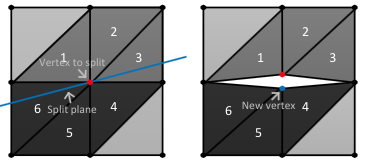
\includegraphics[width=4in,natwidth=366,natheight=166]{img/splitVertex.png}
  \caption
   {Tearing of cloth as presented in \cite{fast_sim_tearing}. The vertex in red is split in two (right). A splitting plane is used to determine how to assign the triangles. Image by \cite{fast_sim_tearing}.}
 \label{fig_split}
\end{figure}

However, the technique described in \cite{fast_sim_tearing} skips over a very important part of the tearing algorithm: how to update the physical representation, i.e. the mass-spring model in this case. In fact, updating the physical representation presents quite a challenge compared to a non-tearable piece of cloth. The student had to figure this out on his own, so the resulting algorithm in the {\bf TearBehaviour} class is for a large part a contribution of the student himself.\\

Practically, it comes down to dealing with the springs in an appropriate way:
\begin{itemize}
\item Some of the springs connected to the split vertex need to be connected to the new vertex. Whether a spring is connected to the new vertex or stays connected to the old one is decided by the direction of the vector between the split vertex and the other vertex on the spring. This is a similar idea to how the faces are divided.
\item Others have to be deleted (especially bending springs that go across the split). Otherwise, the triangles might be no longer connected physically, but there will still be a spring force between them, resulting in unnatural behaviour.
\item Some springs have to be created too, and then added to the cloth: as seen in figure \ref{fig_split}, some triangle edges are duplicated. By only reconnecting the initial springs, some of these duplicate edges won't have structural spring associated with it. We need to create new structural springs for these edges.
\end{itemize}
One interesting question is how long these new springs should be: they can be created with rest length equal to the distance between the particles at that moment, stretching the cloth when it's torn. This mimics the way some materials behave in real-life. Another option is to create the spring with the average rest length of the initial structural springs. This would make the triangles go back to a size similar to their initial size. In the current implementation, I used the latter option, as it looked more natural. In a future development, it might be worthwhile to add a parameter for stretchiness of the cloth.\\

\cite{fast_sim_tearing} describes an altered data-structure to help split the triangles of the mesh, based on a half-edge structure. Unfortunately, their data-structure is, just as the rest of the paper, completely focused on the splitting of the triangles used for rendering, and no mention is made of the physical representation. The authors claim to be neutral to any physical representation, and while this is true, it still leaves some questions unanswered. How can one easily find all springs connected to some particle? How can one represent and find bending springs? In order to have believable tearing it is important to handle all springs related to the split particle in the correct way: springs connected to the split vertex need to be reconnected, bending springs going across the split should be deleted and all face edges should have a spring. All data to do so should be easy to look up.\\

\subsection{Modified Half Edge Structure}

To solve this problem, the student has come up with his own data structure. While the authors in \cite{fast_sim_tearing} were going in the right direction when selecting the half-edge structure, the student has altered the half-edge structure in a different way to include both the triangles (for rendering) and the physical mass-spring model in the structure. This unified structure allows the student to tear the cloth with every look-up in constant time.\\

The structure developed in this project consists of three elements: Vertices, Faces and HalfConnections. In pseudo-code, these elements look like this:\\
\lstset{language=C}
\begin{lstlisting}
struct Vertex {
    HalfConnection random;
    TriFace[] faces;
};

struct HalfConnection {
    HalfConnection next, previous;
    HalfConnection opposite;
    Vertex start, end;
};

struct TriFace {
    Vertex a, b, c;
};
\end{lstlisting}

These elements are pointing to each other in the following way:
\begin{itemize}
\item the element random of Vertex points to one arbitrary HalfConnection that has the Vertex itself as its start element.
\item The faces array of Vertex contains all faces that have the Vertex as one of its three vertices.
\item The elements next and previous of HalfConnection point to the next and previous HalfConnection that have the same start Vertex as this HalfConnection. This is a crucial difference with the original Half-Edge structure: following the next element of a HalfConnection does not take you around a triangle, but takes you around all HalfConnections (and hence springs) that start from the same vertex.
\item The element opposite of HalfConnection points to the (unique) HalfConnection which has this HalfConnections start vertex as end vertex and vice versa.
\item The attributes start and end of the HalfConnection are the vertices at the start and end of the HalfConnection, respectively.
\item TriFace just has three vertices.
\end{itemize}
To clarify, image \ref{structure} shows some of the connections between Vertices and HalfConnections.\\

\begin{figure}[!htb]
  \centering
  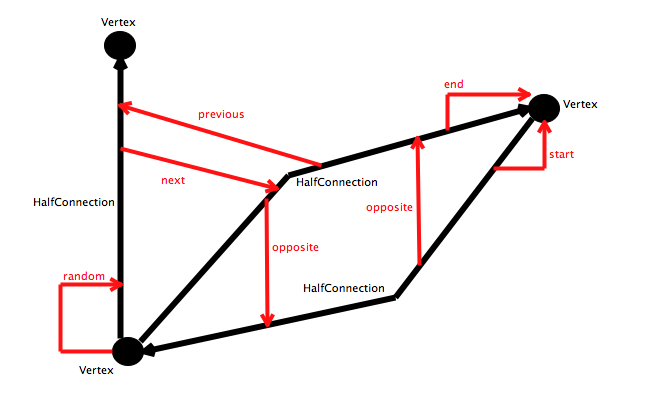
\includegraphics[width=4in,natwidth=366,natheight=166]{img/diagram.png}
  \caption
   {The modified half-edge structure. The elements are in black, the connections between them in red. Note the next (and previous) connection between HalfConnections: connected HalfConnections start at the same Vertex. To be clear: not all connections are in here, just one example of every type of connection.}
 \label{structure}
\end{figure}

The halfconnection and its opposite together, map directly to one spring in the system, connecting two particles (start and end), represented as the Vertex elements in the structure. The cloth is rendered as triangles, which are kept as TriFaces. The difference mentioned in the list, allows to find all springs starting at the same particle easily.\\

It is important to note that the HalfConnections do not represent triangle edges but springs, and as such no longer have a connection to a face, which is a second important difference with the original structure. This allows for bending springs to be added, as they have no natural connection to some face. Furthermore, for our purposes, this connection was not really necessary anyway. The earlier mentioned new definition of the next and previous connection makes it very easy to find all springs connected to a given particle.\\

We can now have a look at what operations this structure allows. For this we assume that in any regular mesh, a vertex is roughly part of the same amount of triangles (e.g. about eight). This assumption means that when the mesh grows (the amount of triangles grows), the vertices will not have more triangles, but more vertices will be added containing more triangles. In other words, we assume the ratio of vertices to triangles to be (almost) constant. This also implies that every particle is connected to a similar amount of springs.\\

If this assumption is true (which is reasonable for most meshes), this structure allows to find adjacent faces to a given face, but also find all springs connected to a given index, check if two particles are connected with a spring, check whether a spring is a bending spring, and several similar checks, all in constant time. For all of its uses, I refer to the {\bf TriangleRenderStructure} class. The constant time look-ups are absolutely necessary for the tearing behaviour, which already has to iterate over all springs. In other words, this structure keeps the tearing within linear complexity. On top of being used for the tearing, it is used in some other places, such as finding adjacent faces in the {\bf ClothFactory} class, and putting the positions into the right order to be rendered as triangles.\\

With this datastructure in place, all necessary look-ups can be done to do the tearing. The overall idea was explained earlier, the exact details of how to reconnect, create and delete new faces and springs can be found in the code in the {\bf TearBehaviour} class.

\subsection{Results}
This section will show some results of the tearing algorithm. Obviously, the accompanying video or the actual software can give a better overview of what the tearing looks like. As with most simulation algorithms, it might require some tweaking of parameters before it looks right.

\begin{figure}[!htb]
  \centering
  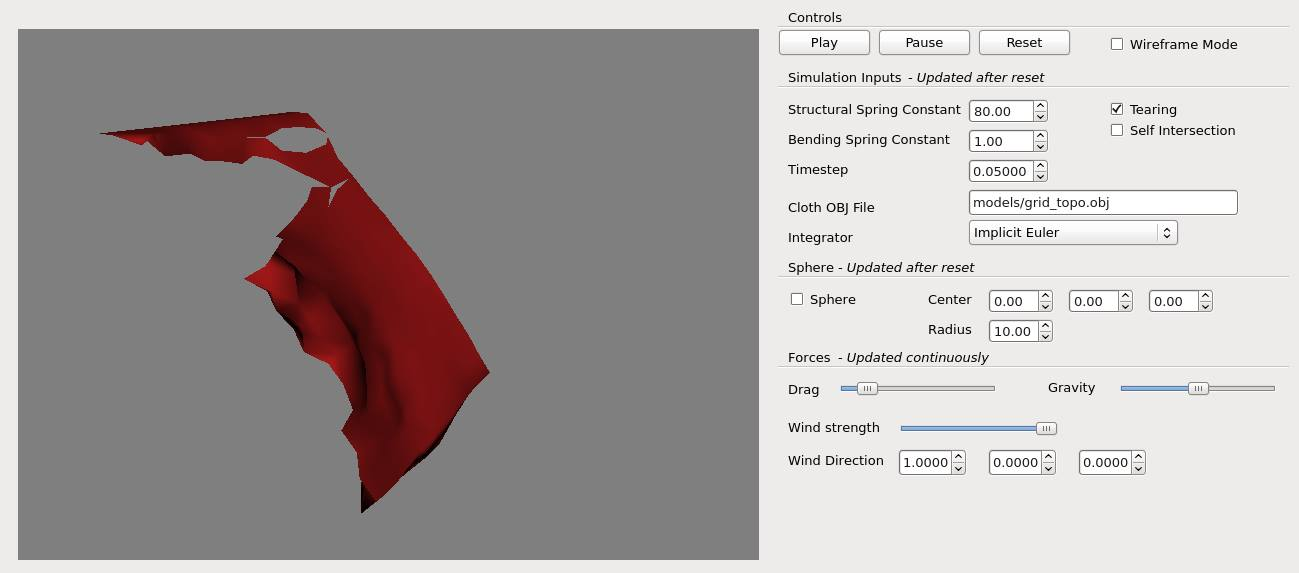
\includegraphics[width=4in,natwidth=366,natheight=166]{img/tornUp1.jpg}
  \caption
   {Example screenshot of the tearing in action.}
\end{figure}

\begin{figure}[!htb]
  \centering
  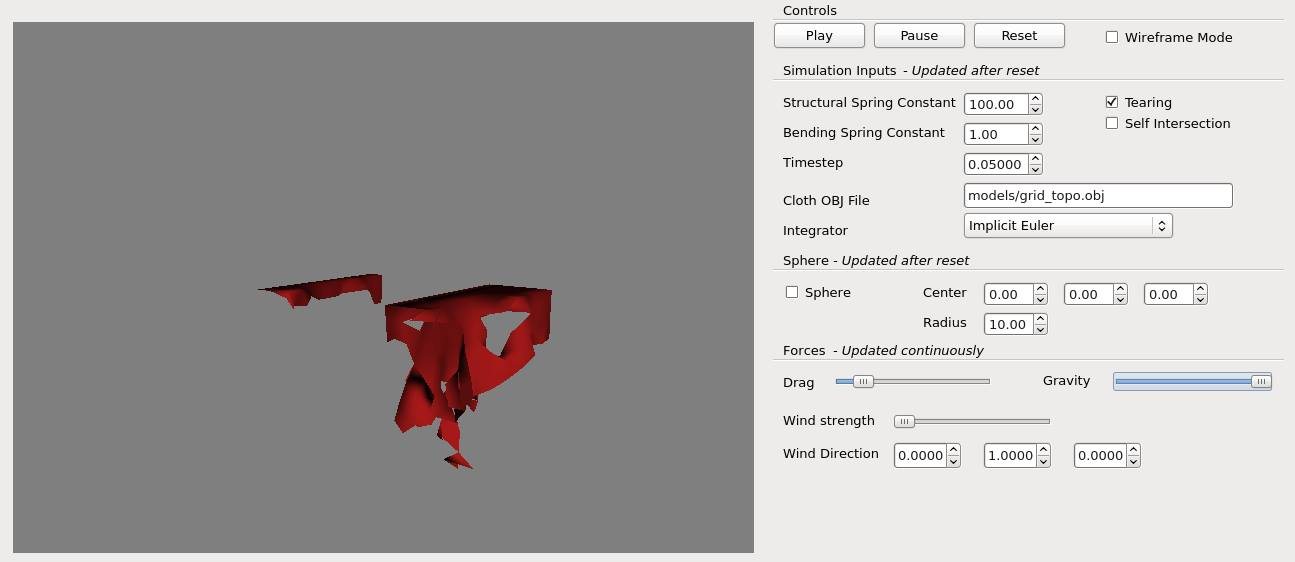
\includegraphics[width=4in,natwidth=366,natheight=166]{img/tornUp2.jpg}
  \caption
   {Example screenshot of the tearing in action.}
\end{figure}


\ifx\isEmbedded\undefined
% References
\addcontentsline{toc}{section}{References}
\bibliographystyle{../ref/harvardnat}
\bibliography{../ref/master}
\pagebreak
\end{document}
\fi